\chapter{Marco de Referencia}

 Desde finales del siglo pasado, los avances tecnológicos en la miniaturización de la electrónica y los componentes mecánicos han allanado el camino para la creación y desarrollo de objetos voladores de pequeñas dimensiones, tales como aviones y helicópteros, los cuales están adquiriendo cada vez más habilidades para realizar vuelos de forma autónoma. Estos dispositivos son popularmente conocidos como drones, un término derivado del inglés \say{abejorros}, y se consideran máquinas voladoras autónomas o semi-autónomas capaces de llevar a cabo misiones de vuelo. En el ámbito internacional, se les conoce como UAVs del ingles \say{Unmanned Aerial Vehicles}, y representan una tecnología compleja cuyo control presenta desafíos, dado que sus características aerodinámicas son similares a las de las aeronaves convencionales \cite{eisenbeiss2004mini}.

El estudio de estos dispositivos despierta un gran interés debido a su versatilidad y capacidad de maniobra, lo que les permite llevar a cabo una amplia gama de tareas en diversas aplicaciones, tales como el uso civil, militar y aeroespacial \cite{nawaz2019applications, shakhatreh2019unmanned, xiaoning2020analysis}. En la figura \ref{fig1_aplicacion_UAV}, se presenta una clasificación detallada de las aplicaciones más importantes de los UAVs.

\begin{figure}[H]
    \centering
    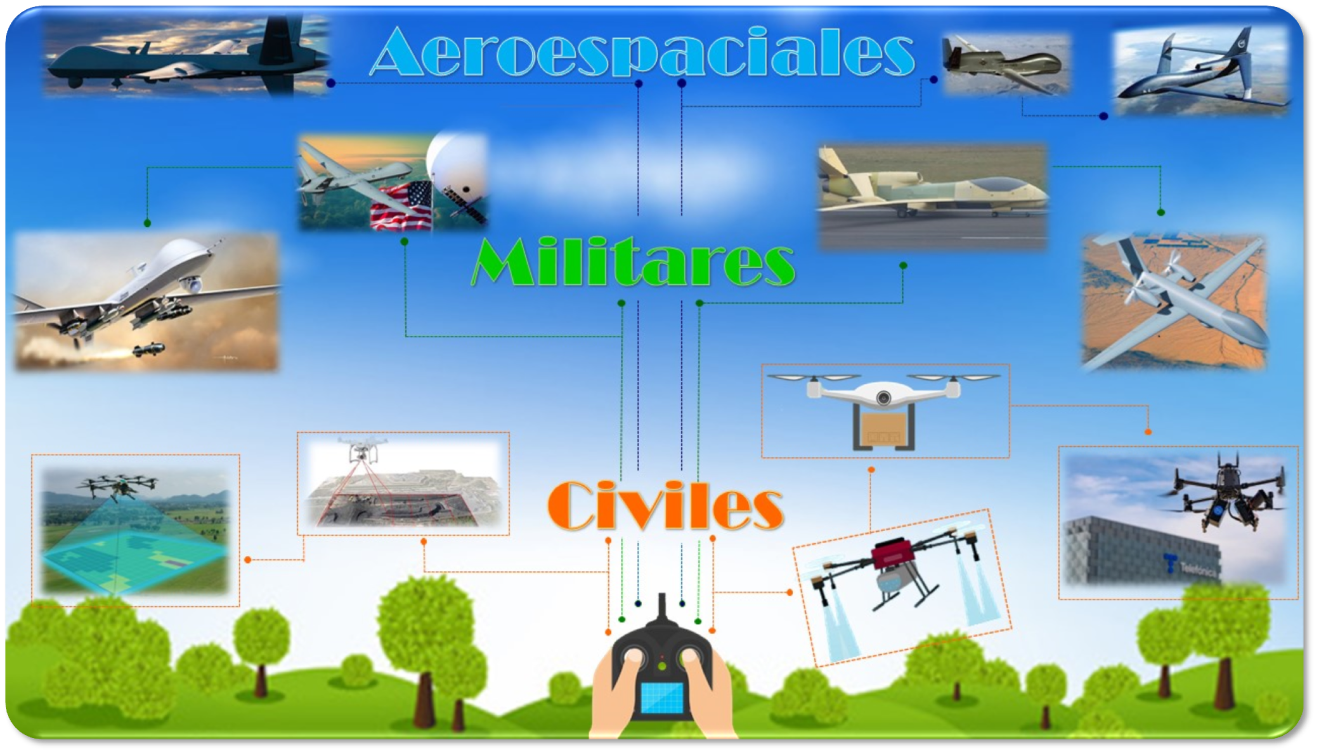
\includegraphics[width=16cm, height=7.5cm]{imagenes/Aplicaciones_UAV.png}
    \caption{Áreas de aplicación UAVS.}
    \label{fig1_aplicacion_UAV}
\end{figure}

\section{Antecedentes.}

Los drones han atraído la atención de la comunidad investigadora que trabaja tanto en el campo militar como en el civil, con una gran cantidad de usos que han sido propuestos por los grupos de investigación, debido a sus características como capacidad y configuraciones, donde el helicóptero de cuatro rotores tiene el mayor número de citas en la literatura de control y ha sido ampliamente investigado para pruebas tanto en interiores como en exteriores . 

\section{Objetivo General}
Desarrollar un sistema web de gestión de inventario y punto de venta para libros, discos y coleccionables, utilizando el framework laravel y arquitectura MVC, con el propósito del control de existencias y la mejora de los procesos administrativos de las sucursales.

\textbf{}
\section{Objetivos Especificos}

\begin{enumerate}
\item Recopilar las necesidades de la tienda para la mejora de la función clave del sistema, como las ventas diarias, la administración de productos y el control entre las sucursales.

\item Diseñar la estructura del sistema mediante el stock tecnológico asignado y el modelo de la base de datos, para la precisión de la información de manera clara, y el buen funcionamiento del sistema.

\item Programar el sistema web utilizando la tecnología necesaria para la gestión de los usuarios, permisos y el catalogo de libros, discos y coleccionables.

\item Crear una interfaz sencilla y visual mediante la integración de componentes intuitivos y flujos de navegación optimizados, para la obtención de un punto de venta ágil y búsquedas de productos rápidas.

\item Ejecutar pruebas de funcionamiento a través de simulaciones de escenarios y pruebas de uso, para la corrección oportuna de errores y la garantía en la exactitud del inventario.



\end{enumerate}

\section{Alcance}


\section{Limitación}

\section{Problemática}


\section{Justificación}

